\chapter{Biomechanics of the Lower Limb as Design Guidelines for Assistive Devices} \label{sec:mimicHSMS}

\section{Introduction}

The concept of mimicking the human skeletal muscle system in soft robotic applications for human assistance was introduced in the previous chapter. This concept relies on a deep understatement of the biomechanics of the human body. Therefore, this chapter presents the investigation performed on the biomechanics of the human lower limb. The main contribution of this chapter is the proposed approach to visually represent the biomechanical data from the human lower limb which can be used as design guidelines for assistive devices. This chapter is structured as follows:
In section two, the terminology relevant to the biomechanics of the lower limb is presented. 


Consider: Merge chapter 2 and chapter 3. Move the work done for the conference paper to the appendix.

In this chapter, the latter concept is further investigated. This concept is mainly basedidentified. The latter concept is based on the mechanical model of the muscle-tendon component. In line with the aims of this research, this chapter is focused on understanding the biomechanics of the human body, specifically of the lower limb due to its great contribution on the Activities of Daily Living (ADLs). Therefore this chapter is divided as follows.
Section one focuses on understanding the terminology involved in the biomechanics of the human lower limb. In section two, many clinical trials, also known as gait analysis, are reviewed to characterize the parameters of torque, angle, and power of the human lower limb during ADLs. Section three describes the muscle-tendon component from a mechanical perspective. Section four introduces many recent works and approaches which attempt to translate the functionality of the muscle-tendon component into soft robotic applications. Section five describes how recent works are addressing the lack of modelling tools for soft materials, considering two main modelling approaches: model-driven and data-driven. Finally, the last section presents a summary of the relevant findings of this chapter.

\section{Characterization of Kinematic and Kinetic Parameters for Activities of Daily Living} \label{sec:characterizationKKP}

The biomechanics of the human lower limb are self-contained between three planes of action, which are the sagital plane, the frontal plane and the transverse (horizontal) plane \cite{PhysicalSolutions2016}. In combination with these planes there are three axes used to identify specific motions: frontal horizontal axis, vertical axis and sagittal horizontal axis. The positioning of each of them is illustrated in \Cref{fig:body_planes_axes}. The sagital plane divides the body vertically into left and right parts, the frontal plane divides the body vertically into front (posterior) and back (anterior) parts and the transverse plane divides the body horizontally into upper (superior) and lower (inferior) parts. This coordinate system allows the many motions of each joint in the human body to be clearly identified.

\begin{figure}[htbp!]
    \centering
    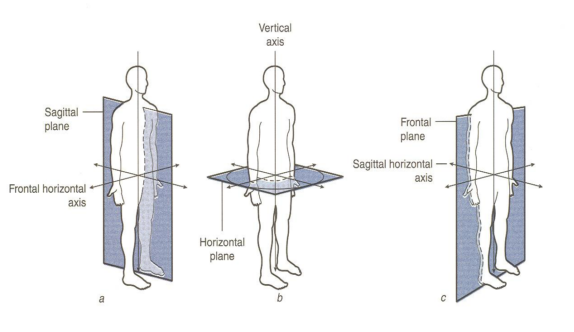
\includegraphics[width=\textwidth]{BoydPlanesAxes.png}
    \caption{Dimensional spaces used to understand human motions: a) Sagittal plane, b)Horizontal plane and c)Frontal plane. \cite{PhysicalSolutions2016}. }
    \label{fig:body_planes_axes}
\end{figure}

\newpage
The motions of each joint are named according to the plane and axis where they happen. This allows the easy recognition of the human body motions (\Cref{fig:lower_motion}). The biomechanics of the lower limb are categorized in five groups, each containing two individual motions, as follows:
\begin{itemize}
    \item Flexion and extension describe the bending motion which decreases, or increases the angle between two parts of the body, respectively.
    \item Abduction and adduction describe the motion away from, or towards the body midline, respectively.
    \item Eversion and inversion of the foot describe the motion away from, or towards the body midline, respectively.
    \item External rotation and internal rotation describe the motion away from, or towards the body midline, respectively.
    \item Horizontal abduction and adduction describe the motion away from, or towards the body midline, respectively.
\end{itemize}

\begin{figure}[htbp!]
    \centering
    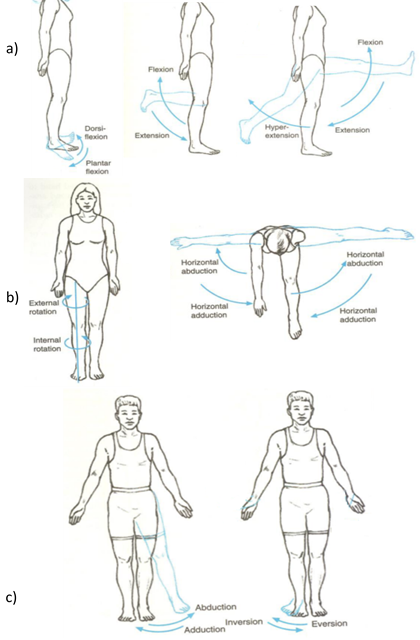
\includegraphics[width=0.8\textwidth]{LowerLimbMotionTerminology.png}
    \caption{Lower limb motions for a) sagital plane, b) horizontal plane and c) frontal plane. Image adapted from  \cite{PhysicalSolutions2016}. }
    \label{fig:lower_motion}
\end{figure}

\newpage

The biomechanics of the lower limb also involves a set of kinetic and kinematic parameters of each joint. The kinematic parameters describe the human body motion in terms of the joint angle, velocity, and acceleration. The kinetic
parameters describe the forces causing this motion, e.g. joint torque and power. Motion capture is the most commonly used method to extract these parameters. However, other technologies such as soft strain sensors \cite{mengucc2014wearable}, electrogoniometers \cite{wu2011electromyography}, and inertial measurement units (IMU) have also been used. The process of characterizing these parameters is very important for the development of any wearable robotic device. This allows the intended device to be tailored for a specific application, it being assisting an elder adult or enabling a disabled subject to move. Alternatively, the kinetic and kinematic parameters can be also used to measure the effectiveness and compatibility of an already available assistive device. Measuring the effectiveness of an assistive device in this way is more convenient than calculating the metabolic cost reduction, which involves specialized equipment \cite{panizzolo2016biologically}. 

The kinetic and kinematic parameters can be obtained from gait studies. These studies differ between one another in many aspects, in addition to the technology of choice, such as subjects' gender, age, weight, etc., as well as the setup of the experiments. Therefore, the following subsection describes the process of extracting and digesting the kinetic and kinematic parameters from gait studies. As previously mentioned, these parameters are useful design guidelines for wearable robotic devices. The gait studies compiled in the following section cover the main activities of daily living (ADLs), which are: walking, ascending/descending stairs, ascending/descending ramps and chair sitting down/standing up. In the context of studying the human lower limb, the joints of interest are the hip, knee and ankle joints.

\subsection{Gait Analysis Data}

In clinical studies focused on analyzing the human gait, parameters regarding the subjects involved and the experiment performed are commonly provided. Regarding the subjects characteristics, information about their age, subject age, weight, height, gender and health condition are included. Similarly, contextual information about the experiment performed such as: loading conditions, plane geometry, and activity of choice is provided. Subjects characteristics are always presented in mean values with the respect to the whole group participating. In a similar way, measured and calculated data, such as torque and power, is presented in mean normalized values. The gait cycle is usually normalized using the subjects height, whereas the joint torques are normalized using the subjects weight. The latter is clearly expressed in the units of the reported values, being Nm/kg for the joint torque, and W/kg for the joint mechanical power. Nonetheless, some studies do not follow the same guidelines when reporting the obtained results, or when normalizing the calculated values, preventing the reported information to be compared against other clinical studies \cite{lee2008biomechanics}. 

The diversity on the subjects characteristics difficult the comparison process against similar clinical studies. Due to this, some clinical studies focuses on studying a common characteristic among all participants, such as age or health condition. This is the case for the performed in \cite{bovi2011multiple}, where the study group is segmented in two age groups. One group included subjects from 22 to 72 years old, meanwhile, the subjects from the other group have ages ranged from 6 to 17 years old. With this segmentation approach, the clinical study can present the results with respect to age range. In some cases where the difference between age groups is very small, the clinical study condense the reported data into a single dataset \cite{lee2008biomechanics}.

The technology of choice to extract the kinematic parameters of the human gait, such as the joint angle, is motion capture. Similarly, the human body kinetics parameters are extracted by measuring the ground reaction forces using force plates. The latter is required to calculate the joint torque and joint power. Therefore, the three most common parameters found in gait analysis studies are the angle, torque, and power of the joint of interest. The gait cycle of the studied activity is usually presented in a chart accompanied with tables to clearly indicates the maximum, minimum and mean values of the gait cycle. The difference between the maximum and minimum values of the kinematic and kinetic parameters of a gait cycle are very important for the characterization process. Commonly, these values are provided in the studies in the form of tables and charts \cite{han2011biomechanical,yali2010biomechanics}, in other cases the complete experiment dataset is included \cite{moore2015elaborate}. The extraction of the parameter of interest is straightforward when the data is presented in a form of a table. Alternatively, when data is provided in the form of charts, the process of extracting it must be done by visual inspection, which inherently add some degree of error to the extracted value \cite{protopapadaki2007hip,riener2002stair,mcintosh2006gait,roebroeck1994biomechanics,mak2003joint}. Likewise, it can be the case for some studies to focus on specific features of the gait cycle, such as maximum and minimum values of each parameter; or not provide one or more of the parameters of interest (angle, torque or power). Due to all these different scenarios, the process of curating and compiling the data found in clinical studies is very lengthily. The latter motivated the process described in the following section in which the data of several clinical studies is compiled and visually presented to serve as design guidelines for the development of soft robotic applications for human assistance.

\subsection{Extracting Design Guidelines FIIIIIIIIIIIIIIIIIIIIIIIIIIIIIIIIIIIIIIIIIIIIIIIIIIIIIIIIIIIIIIIIIIIIIIX}

Add introductory paragraph to this section.

The variations of the data from one experiment to another can be reduced by focusing on the range obtained from the difference between the maximum and minimum values of each parameter. This is illustrated in \Cref{fig:HipKKPWalking}, despite the variations between the maximum and minimum values from one experiment to another, the actual range of each parameter is similar among all the experiments. The mean range of motion for the hip joint angle throughout different walking over-ground experiments was found to be 44.63\degree{} (\Cref{fig:HipKKPWalking}). Also, the greatest variation between the mean range value and the range value of each experiment is 18\% of the mean value. The previous calculation can be used to decide design parameters of wearable robotic devices, such as which range of motion should be covered by the device depending on which sector of the population is intended to be assisted. Alternatively, the device can be tailored to cover as much of the population as possible by choosing the maximum and minimum values of the range of motion, out of all the experiments. 
\begin{figure}[htbp]
    \centering
    \begin{subfigure}[b]{0.75\textwidth}
        \centering
        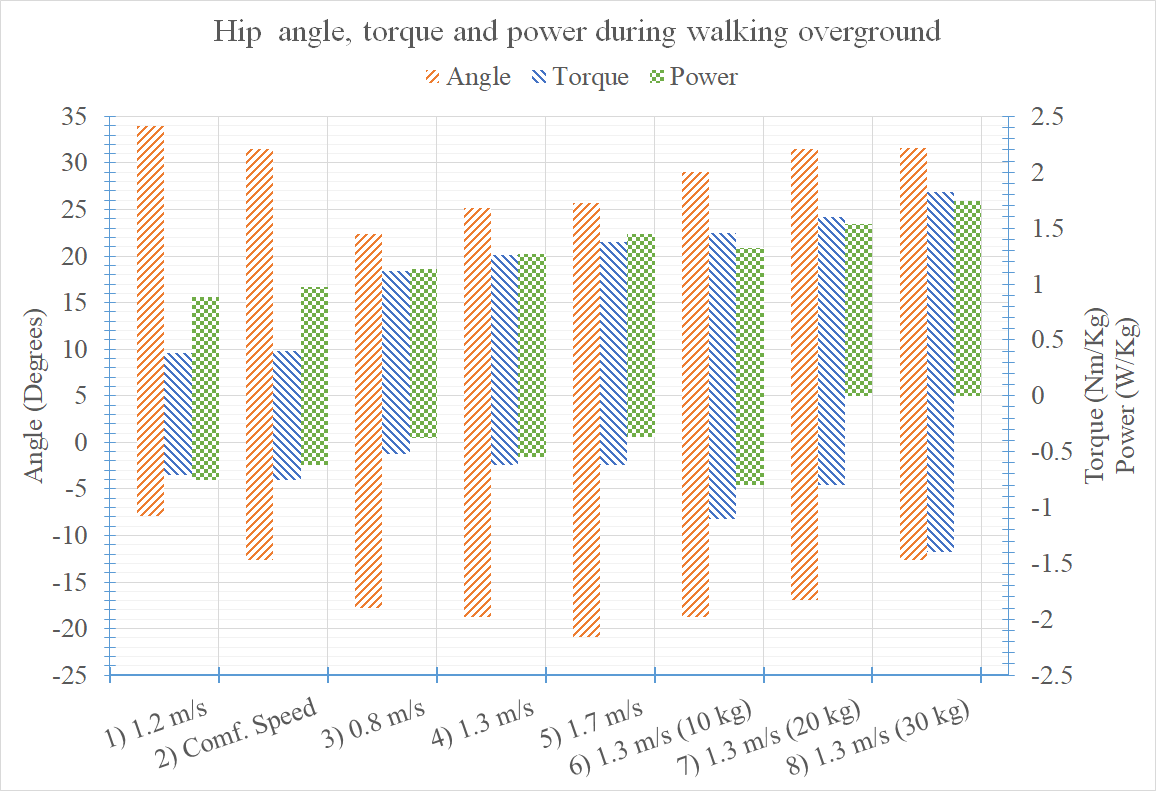
\includegraphics[width=\textwidth]{HipKKPWalkingExcel.png}
        \caption{Hip joint characteristics for walking over ground activities. The weight next to the name of some activities dictates the load carried by the subjects during the experiment \cite{solis2017characterization}. Data collected from: (1) \cite{bovi2011multiple}, (2) \cite{lee2008biomechanics}, (3-8) \cite{han2011biomechanical}. }
        \label{fig:HipKKPWalking}
    \end{subfigure}
    \hfill
    \begin{subfigure}[b]{0.75\textwidth}
        \centering
        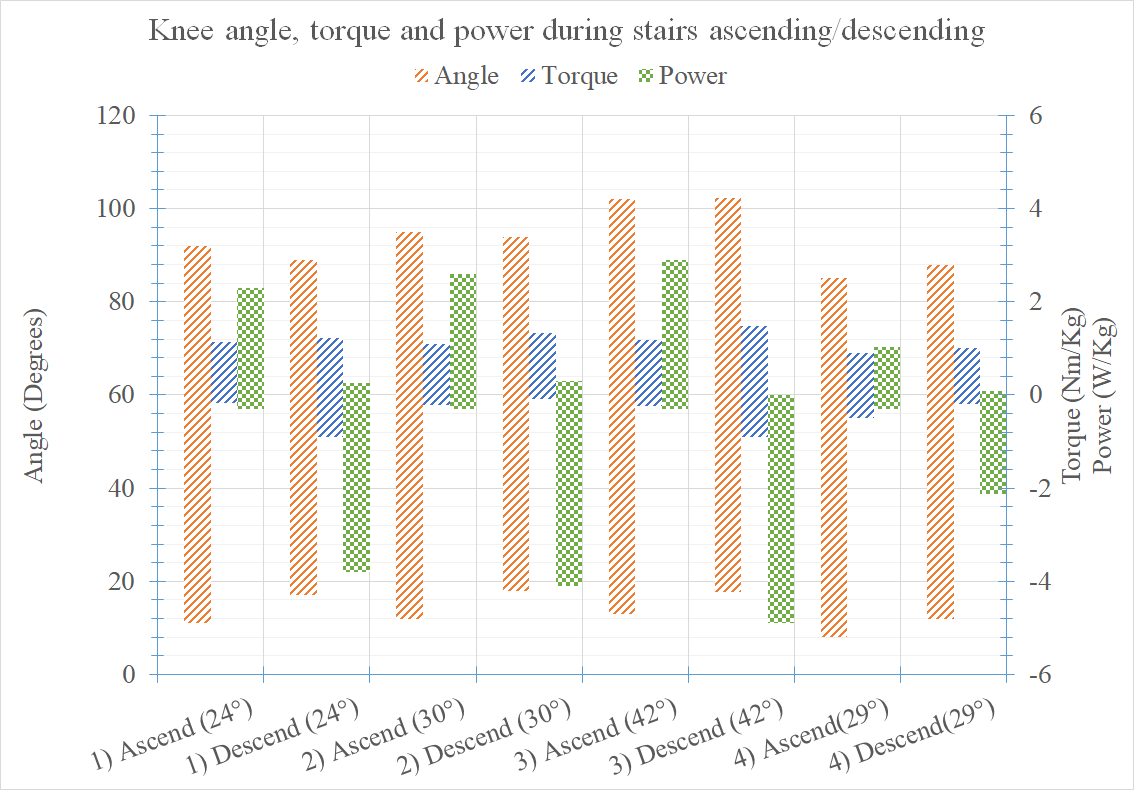
\includegraphics[width=\textwidth]{KneeKKPStairsExcel.png}
        \caption{Knee joint characteristics for several stairs ascending/descending experiments. The number enclosed in brackets represents the stairs slope. Data collected from: (1) \cite{riener2002stair}, (2-4) \cite{reid2007knee}. }
        \label{fig:KneeKKPWalking}
    \end{subfigure}
    \caption{Clustered-stacked bar charts of reviewed gait analyses \cite{solis2017characterization}. }
    \label{fig:clusteredMain}
\end{figure}

Different design guidelines can be extracted when visually analyzing other parameters together. For example, in \Cref{fig:KneeKKPWalking} , the parameters of the knee joint are now compared against many experiments of stairs ascending/descending. Now, the main feature is not the range of motion of the knee, but the characteristics of the torque values. They appeared mirrored, in other words, the torque values required for descending stairs are of similar magnitudes but opposite in direction. Also, the amount required for ascending stairs is generally twice as much as the amount required for descending stairs. The latter illustrates an optimization opportunity. When designing a wearable robotic device for human assistance, the actuator is chosen to satisfy a certain torque range of a particular activity. Without the characterization of the parameters performed, the actuator is most likely to be oversized to comply with the most demanding part of the activity. However, a different approach could be proposed: agonist-antagonist actuators; a technique implemented in several wearable robotic devices which at the same time complies with the actual functionality of the human skeletal muscle system.

Another useful way of extracting design guidelines from the gait analyses is to plot the range of a specific parameter against different ADLs. To the best of the author's knowledge, this approach has only been documented once in \cite{rowe2000knee}, where the range of motion of the knee joint is compiled into a chart for 11 different ADLs. This concept, illustrated in \Cref{fig:HipTorqueRange}, can provide insight of two important design parameters. On the one hand, the actuators meant for this application must be able to deliver torques in both directions of rotation, i.e. clockwise and anti-clockwise. On the other hand, the selected actuation technology must meet the torque requirements of the activity of interest, illustrated in \Cref{fig:HipTorqueRange}. \Cref{fig:HipTorqueRange} was constructed using the mean range of the hip joint torque during different activities \cite{bovi2011multiple,lee2008biomechanics,han2011biomechanical,protopapadaki2007hip,riener2002stair,mcintosh2006gait,roebroeck1994biomechanics,mak2003joint}.

\begin{figure}[htbp!]
    \centering
    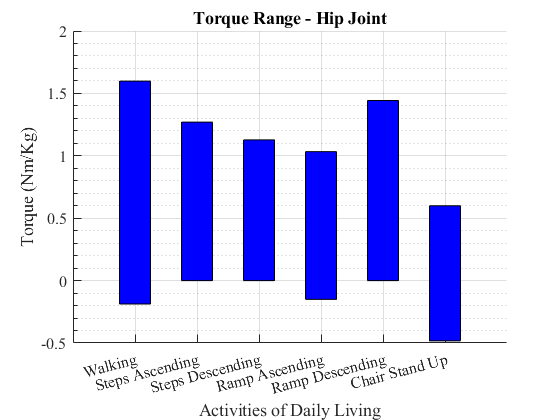
\includegraphics[width=0.8\textwidth]{HipTorqueRange.png}
    \caption{Torque range values during several activities. The values for the maximum and minimum torque are mean values from the data of all the different gait analysis experiments enclosed in one main activity. \cite{bovi2011multiple,lee2008biomechanics,han2011biomechanical,protopapadaki2007hip,riener2002stair,mcintosh2006gait,roebroeck1994biomechanics,mak2003joint,solis2017characterization} }
    \label{fig:HipTorqueRange}
\end{figure}

Another alternative of visual representation of the data can be done by grouping the range of a specific parameter and comparing it with any of the subjects' physical characteristics, e.g. the age range. This is illustrated in \Cref{fig:KneeRangeAge}, where the dependency of the subjects' age with the knee range of motion is evidenced. The colour code used in \Cref{fig:KneeRangeAge}, the age ranges and knee ranges of motion are presented in \Cref{tbl:KneeRangeMotionage}. The chart shown in \Cref{fig:KneeRangeAge} concentrates the data from three different gait analyses, in which six age groups are contained. The approach used in \Cref{fig:KneeRangeAge} is to overlap areas of different colours, each area represents the range of motion of the knee for a specific age range. The area in which several areas intersect can be appreciated due to the enabled transparency property. Nevertheless, the areas where three and two areas are intersected are manually highlighted by a surrounding solid line and dotted line respectively, to improve their visualization. This simple intersection of areas can provide information regarding the required range of motion to be delivered by the wearable robotic device, depending the sector of the population focused on.
For example, if a wearable robotic device was aiming to assist the population sector aged from 50 to 70 years old, then a range of motion of the knee joint from 5{\textdegree} to 63{\textdegree} would be enough to cover the mentioned population. The range of motion is taken from the triple intersection of areas illustrated in \Cref{fig:KneeRangeAge}, which can provide a certain degree of confidence since three different clinical studies were compared. This approach can be used to compare other characteristics, e.g. subject's weight against torque. Summarizing, the areas overlapping approach can provide guidelines to avoid oversizing of the wearable robotic device to be developed by analysing the intersection of different areas which ultimately provides a degree of confidence when deciding design parameters.

\begin{table}[htb!]
\caption{Colour code used in \Cref{fig:KneeRangeAge} for each combination of age range and knee range of motion  \cite{solis2017characterization}.}
\label{tbl:KneeRangeMotionage}
\begin{tabular}{c|c|c|c}
\hline
Colour Code & Knee Range of Motion (\degree{}) & Age Range (Years) & Clinical Study \\
\hline
Red         & 2.2 - 67.4               & 49 - 90           & \cite{rowe2000knee}       \\
Green       & 5 - 66.5                 & 6 - 17            & \cite{bovi2011multiple}        \\
Blue        & 4.5 - 63.5               & 22 - 72           & \cite{bovi2011multiple}           \\
Yellow      & 0 - 69                   & 18 - 30           & \cite{lee2008biomechanics}        \\
Magenta     & 0 - 69                   & 50 - 70           & \cite{lee2008biomechanics}     \\
Cyan        & 8 - 63.6                 & 23 - 27           & \cite{han2011biomechanical}    \\  
\hline
\end{tabular}
\end{table}

\begin{figure}[htb!]
    \centering
    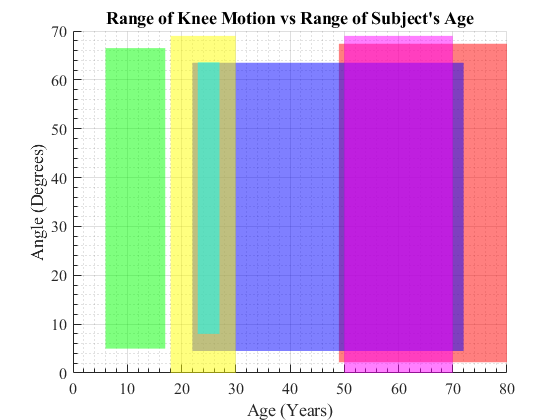
\includegraphics[width=0.7\textwidth]{KneeRangeMotionAge.png}
    \caption{Comparison between subjects' age and the knee range of motion during walking over ground. The areas surrounded by solid lines and dotted lines represent the intersection between three and two areas, respectively. The overlapping squares highlight the great similarity among the range of motion despite subjects' age. The data used to create this chart is presented in \Cref{tbl:KneeRangeMotionage} \cite{solis2017characterization}. }
    \label{fig:KneeRangeAge}
\end{figure}

In this section the process of characterizing the human lower limb kinematics and kinetics parameters during some ADLs was described. The relevant information provided in gait analysis experiments, and the challenges faced when extracting it from the clinical trials, were described. Data compiled for the activities of walking, ascending/descending stairs, ascending/descending ramps and chair standing up were presented in the form of clustered stacked bar charts. This type of chart allowed quick and easy detection of similarities between several clinical trials of the same activity. In contrast, the spotted differences, as the ones for the knee torque values during ascending/descending stairs, are indicators for optimization opportunities where instead of using a single actuator to satisfy the torque range, an agonist-antagonist system could be more suitable.

The reliability of the data can also be observed using the type chart of overlapping areas with subjects' ranges of age against the knee ranges of motion. In other words, the specific ranges in which the data from different experiments overlaps, gives a measure of consistency which can be used to tailor the developed wearable device coverage. 

The chart style with ranges of motion versus activities, facilitates the choice of the actuator type and dimension (depending on the activities of interest). The styles used to represent the charts were kept as simple as possible while providing useful information about the KKP. However, more complex plotting methods can be used. Finally, a total of 12 charts were produced in Excel\textregistered{} using the compiled data from the gait analyses. In favour of keeping the length of this section adequate, only two out of the 12 charts were included in here. The remainder charts were moved to \Cref{appendixA}.

\section{The Muscle-tendon Component} \label{sec:muscle_tendon}

Having defined the terminology involved in the biomechanics of the human skeletal muscle system, and characterized the kinetic and kinematic parameters of its lower limb, this section focuses on describing the muscle-tendon component from a mechanical point of view. 

In the literature, the mechanical model commonly used to describe the mechanical behaviour of the muscle-tendon component is the Hill's model \cite{hill1938heat}. This model is considered to be the most representative of all the available models \cite{zhang2012sma}. Hill's model describes the skeletal muscle as a three elements system, which contains a contractile element, a passive element, and a series element. The contractile element (CE) represents the muscle fibres in charge of generating the contractile forces, the parallel (passive) element (PE) is formed by the tissue surrounding the muscle which prevents it from overstretching, and the series element (SE) represents the human tendon, as illustrated in \Cref{fig:hillModel}.

\begin{figure}[htb!]
    \centering
    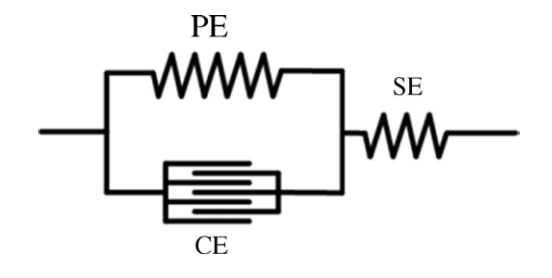
\includegraphics[width=0.4\textwidth]{HillModel.png}
    \caption{Hill's model of the skeletal muscle. The contractile element (CE), the parallel element (PE) and the series element (SE) are shown \cite{hill1938heat} }
    \label{fig:hillModel}
\end{figure}

Hill's model makes the important assumption of considering the SE to be purely elastic, i.e. the deformation of the element is entirely dependent on the force applied to it. Nevertheless, the non-linear viscoelastic properties of the human tendon are acknowledged in his work. The latter simplification is a common practice among studies of the skeletal muscle system because the muscle and tendon are studied as a whole (muscle-tendon component) \cite{zajac1989muscle}. Evidence of the actual benefits of this simplification is found in the literature for the field of robotics exoskeletons. The complex muscle-tendon model developed in \cite{lloyd2003emg}, considered the viscoelastic properties of the human tendon to estimate forces and joint torques in real time. The model achieved high accuracy at the cost of high computational load. In an attempt to reduce the computational load, the assumption of an infinitely stiff tendon was made which proved to be reliable as well \cite{sartori2009stiff}.

In a similar way, developments in the field of soft robotics which are inspired in the skeletal muscle system functionality are also based in Hill's model, as highlighted in \Cref{sec:SoftActuation}. Commonly, springs \cite{park2011bio} or Bowden cables \cite{Zhang2013a} are implemented as the SE of the muscle-tendon model. Nevertheless, the fact is that the human tendon has viscoelastic properties \cite{maurel1998biomechanical}. At the time of starting this research, the documented works in the literature were mainly focused on developing and testing soft materials to be used as the contractile element in soft artificial muscles. The latter, previously identified as a research opportunity, indicates that the viscoelastic properties of soft materials have not been studied with the aim of developing a soft artificial tendon, which in combination with current soft artificial muscles could deliver better performance in soft robotic applications for human assistance.

The first step towards the investigation on the potential benefits of adding viscoelasticity, in the form of a soft SE, to soft actuators is described as follows. As a starting point, the mechanical properties of the human tendon must be investigated. Due to the large contribution of the knee joint in the ADLs, the present investigation is focused in this joint of the human lower limb. Subsequently, the selection and characterization of many soft materials with mechanical properties similar to the human tendon, is proposed. The extracted properties from the studied soft materials and from the human tendon are compared against each other. This comparison analysis has the potential of providing evidence on the benefits and disadvantages of implementing a viscoelastic element as the way to transmit tensile forces in soft orthoses and soft exosuits.

Tendons are connective tissues that link muscles with bones. They have a non-linear viscoelastic behaviour, i.e. the proportional relationship between the reaction force experimented by the tendon and the applied deformation is not constant throughout the whole range of possible deformations. This reaction force is also dependent on the history of previous deformations. At rest, the collagen fibres (core components of tendons) are in a relaxed wavy state. When the tendon experiences a tensile force, the collagen fibres are easily stretched and realigned, opposing little resistance to deformation. However, when the collagen fibres are completely stretched they begin to offer more resistance to deformation which is proportional to the applied force. Finally, fibres can be stretched to their limit and failure of the tendon will occur \cite{nordin2001basic}. This non-linear response to the applied deformation is better explained using \Cref{fig:tendonSS} where the characteristic S-shape curve for tendon stress-strain graph is appreciated.

\begin{figure}[htb!]
    \centering
    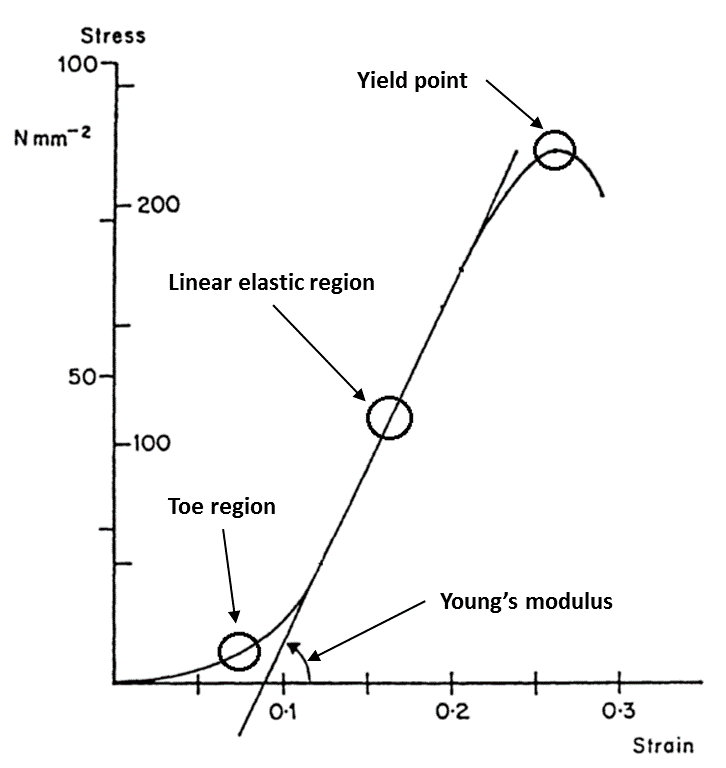
\includegraphics[width=0.6\textwidth]{TendonStressStrain.png}
    \caption{Tendon stress-strain curve. Image adapted from \cite{maurel1998biomechanical}. }
    \label{fig:tendonSS}
\end{figure}

The stress-strain curve in \Cref{fig:tendonSS} illustrates the mechanical properties of a human tendon. The stress is described as the tensile force per cross-sectional unit area experienced by the tendon. This stress causes the tendon to elongate (deform). In the chart, the elongation is represented as the strain, which is the tendon deformation in relation to its original length. Along with the stress-strain curve, the force-elongation curve is also used to visualize the mechanical properties of tendons. These experiments are performed in a static state, i.e. the strain rate is the same throughout the whole experiment. Therefore, they do not provide any information about the viscoelastic properties of the tendon.

Viscoelastic materials exhibit both elastic and viscous characteristics. Viscosity describes a fluid's resistance to flow, the more viscous a fluid is, the more slowly it will flow and vice versa. The latter suggests a time-dependent behaviour. In the case of viscoelastic materials, this time-dependent behaviour is shown when subjecting the material to different rates of strain or deformation. For example, the stress-strain curve of the human tendon, illustrated in \Cref{fig:tendonSS}, would have a greater slope in the elastic region if a greater strain rate is applied. The viscoelastic behaviour of the human tendon can be analysed with the following mechanical tests: stress relaxation, creep (deformation over time) and hysteresis \cite{nordin2001basic}.

During the stress relaxation experiment, the tendon is subjected to a constant deformation (length remains the same throughout the whole experiment). To avoid plastic deformations, i.e. incorrect measurements, the parameter of deformation for this experiment must not exceed the linear region of the material. The initial force/stress triggered as a response of the applied deformation will decrease over time (relax) until reaching equilibrium. From this experiment a chart of force against time is generated (\Cref{fig:tendonSR_Creep}). In a similar way, in the creep experiment a constant force, avoiding plastic deformations, is applied to the material. The material will creep as time passes, in other words, the deformation caused by the applied force will increase over time until reaching equilibrium. A chart of deformation against time is generated (\Cref{fig:tendonSR_Creep}). Finally, during the hysteresis experiment the tendon is subjected to cyclic tests where a load is applied up to a certain stress level and then released (unloading). The tendon behaviour shows two different paths, one for loading and one for unloading. Due to the time-dependent behaviour of viscoelastic materials, each cycle will generate different load-unload paths since the time interval for each cycle to be executed are intentionally defined to prevent the material of reaching equilibrium (\Cref{fig:tendonHysteresis}).

\begin{figure}[htb!]
    \centering
    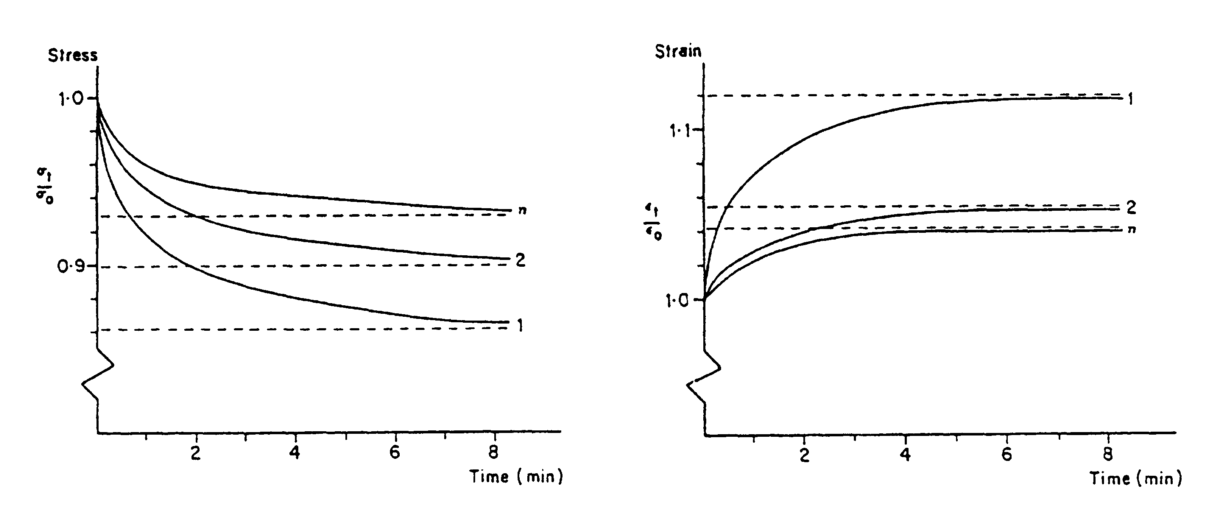
\includegraphics[width=\textwidth]{TendonSR&Creep.png}
    \caption{Tendon curves for the experiments of: (a) stress relaxation and (b) creep. The experiments were executed several times under the same conditions, the curve labelled \textit{n} illustrates the tendon reaching a steady state where repeatability between experiments is achieved. Image reproduced from \cite{maurel1998biomechanical} }
    \label{fig:tendonSR_Creep}
\end{figure}

\begin{figure}[htb!]
    \centering
    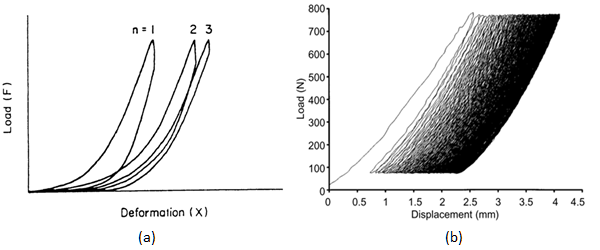
\includegraphics[width=\textwidth]{TendonHysteresis.png}
    \caption{Hysteresis of the human tendon. (a) Deformation chart shows both loading and unloading paths for few cycles and (b) displacement chart shows 200 loading-unloading cycles. The preconditioned state of the tendon is reached for cycles above 50. Images taken from \cite{maurel1998biomechanical,schatzmann1998effect} respectively. }
    \label{fig:tendonHysteresis}
\end{figure}

When performing mechanical experiments to find the tendon properties at failure, the obtained results are different between a preconditioned and an unconditioned tendon, as proved in \cite{schatzmann1998effect}. This effect is illustrated in \Cref{fig:tendonSR_Creep} as well, for both experiments, the tendon relaxation and creep are smaller for each new testing cycle until reaching an equilibrium state, i.e. the preconditioning state. The previous set of experiments is useful to characterize the non-linear viscoelastic properties of tendons and soft materials. Therefore, to perform the comparison analysis mentioned in \Cref{sec:muscle_tendon}, the soft materials of interest must be characterized using some of these mechanical tests. The study of the creep and hysteresis is out of the scope of this research. Instead, the tensile strength and stress relaxation are analysed. The selection criteria for the synthetic soft materials to be used is explained in the next section.

\section{Soft Materials to Match the Properties of the Human Tendon} \label{sec:softMaterials}

The selection of the soft material to be implemented was based on the literature about tendon reconstruction applications. A comprehensive review about the usage of synthetic materials in tendon reconstruction is made by Andullah in \cite{abdullah2015usage}, where the most common materials used as artificial tendons and for tendon reconstruction are reported as: carbon, polyester, polytetrafluoroethylene, among others. The latter suggest that polymers are highly compatible with the human skeletal system and have similar mechanical properties as the human tendon. This assumption is further verified in the study performed by Duenwald et al. in \cite{duenwald2009viscoelastic}, which is about the viscoelastic relaxation and recovery of the human tendon. In this work, a high density polyethylene material was tested to find great similarities between this material and the mechanical properties of the human tendon. In fact, the viscoelastic properties of the human tendon during loading and unloading are similar to the ones found in polyethylene. However, high density polyethylene is not able to sustain high strains without suffering plastic deformations nor it has a very fast elastic response.

Among the current developments in soft orthoses, silicone rubber is a common choice, due to its high compliance, high elasticity and softness. Silicone rubber is usually implemented to create inflatable elements, but it is also known to have non-linear elastic properties, as reported in \cite{roylance2008mechanical}. These findings suggest that the limitations of polymers, in terms of their elasticity, could be circumvented when combined with elastomers, such as rubber. A material with the latter characteristics, is known as a composite material. Many composite materials are created by injecting polymer particles, such as the previously mentioned polyethylene, into a rubber mixture. Thanks to the advances in manufacturing of composite materials, there is a wide variety of commercially available materials that fit with the requirements of this research. Due to the latter information, the selection of the soft materials to be studied in this work are from the family of composite materials, as follows: Polyethylene Rubber, Ethylene Polypropylene, Natural Rubber with Polyester, Natural Rubber, Silicone Rubber, Fluorocarbon Rubber, and Nitrile Rubber. All the materials were acquired from RS Components UK\textregistered{}, with the exception of the Natural Rubber, which was acquired from CoreZone Sports\textregistered{} in the form of resistance bands of different thickness. Finally, the characterization process and more details about the materials are provided in \Cref{ch:characterizationSoft}.

\section{Modelling Techniques for Soft Materials} \label{sec:modelingTechniques}

In \Cref{sec:gaps}, the lack of a reliable model to predict the mechanical behaviour of soft materials was identified as a gap in the body of knowledge. This limitation plays a crucial role in the process of investigating the potential benefits of mimicking the human skeletal muscle functionality, and so it is addressed in this section. 

Most of the documented soft robotic applications use soft materials from the family of thermoplastic elastomers (TPE). These type of materials are known to have a non-linear stress response, low stiffness, high deformation lengths, and a time-dependent and temperature-dependent response \cite{Bauman2008}. These mechanical properties are similar to the ones found in biological skin or muscle tissue, which is why soft materials are being implemented in soft robotic applications, despite of the many challenges. However, it is imperative to have a reliable modelling technique to fully take advantage of the latter mechanical properties.

At this point, it has been established the complexity of the mechanical behaviour of soft materials, such as TPE. In general terms, the stress response of these materials is non-linear and viscoelastic. The most commonly modelling technique used when dealing with viscoelastic materials is the development of a mathematical constitutive model. Many authors, choose the Linear Viscoelastic Models (LVM) as the starting point \cite{xu2014mathematical,tirella2014strain,lu2017constitutive,ciniello2017identifying}. This has also been the case when modelling the mechanical behaviour of biological tissues \cite{sanjeevi1982viscoelastic}. The LVM are a set of mathematical models which use two basic components, a spring and a damper, in different configurations and quantities to describe the viscoelastic mechanical behaviour of materials \cite{roylance2001engineering}. Inside this family of mathematical models, there are a couple of them which are considered able to describe the viscoelastic behaviour of any material, as long as the required number of parameters of the model is met. This immediately imposes the restriction of having enough computational power to deal with the model complexity when high accuracy is required.

At this stage of the research, the implementation of soft materials in soft robotic applications for human assistance has gained more attention. Most of the efforts are focused on improving the traditional series-elastic actuator (SEA) by replacing its elastic element, commonly a metallic spring, with a viscoelastic material, such as rubber. SEA are from the family of cable-driven actuators and are commonly based on electric motors. The main feature of these actuators is that they have an elastic element between the actuator and the load. SEA have greatly impacted the field of robotics, specifically in legged robotics and powered orthoses, due to many benefits such as: greater shock tolerance, low output impedance, passive energy storage, and better force feedback accuracy \cite{pratt1995series,pratt2004series,au2008powered}. Almost two decades after Pratt et al. documented the first SEA prototype, SEA are now considered a mature actuation technology, and as such, they have a well-defined trade-off, caused by the fixed stiffness provided by linear springs traditionally used. More often than not, variable stiffness is more suitable for legged robots and powered orthoses. The latter limitation have been addressed by developing variable stiffness actuators \cite{groothuis2012vsaut}, using non-linear metallic springs \cite{migliore2007novel}, and very recently by using viscoelastic materials, such as polymers and rubber \cite{rollinson2013design,parietti2011series,schepelmann2014compact}. However, these works, specifically the ones dealing with soft materials, are still facing the challenge of modelling the mechanical properties of this type of materials. 

In \cite{parietti2011series}, where the concept of a series-viscoelastic actuator (SVA) is first mentioned, the modelling of the soft material is based on the Burger Model, one of the most complete LVM, in combination with a controlling technique known as the state space observer. The accuracy of the system was found to be proportional to the complexity of the mathematical model used. The studied material in this work was a rigid-acrylic based photopolymer (FullCure720). The reported control system contained the viscoelastic model, the state space observer, and a cascaded force-velocity scheme, in other words, a very complex and well thought control system for a linear viscoelastic polymer. The developed SVA is illustrated in \Cref{fig:firstSVA}. 

\begin{figure}[htb!]
    \centering
    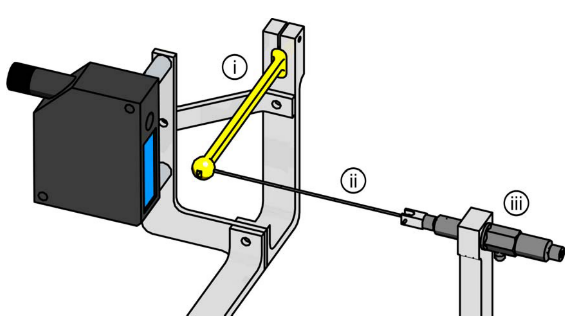
\includegraphics[width=0.6\textwidth]{FirstSVA.png}
    \caption{Series-viscoelastic actuator proposed by Parietti et al. The end-effector is rigidly mounted on the revolving lever (i), which also supports the laser sensor. A Nylon line (ii) connects the end-effector handle to the high-precision piezoelectric force sensor (iii), which is fixed to a rigid support \cite{parietti2011series}.}
    \label{fig:firstSVA}
\end{figure}

Following this line of research, Rollinson et al. attempted to add viscoelasticity to a SEA, this time a soft material is used, natural rubber, instead of a rigid polymer \cite{rollinson2013design}. The developed SEA has a rotary spring. Two different types of rubber, and a type of neoprene, were studied. In here, the stress response of the materials is considered linear and instead, the hysteresis of the material is modelled. Again, the modelling of the soft material is based on one of the LVM, the Standard Linear Solid (SLS) model, which is slightly less complex than the Burger model. Thanks to the proposed mechanical design for the rotary SEA, the reported stress response of the studied rubbers was surprisingly linear under a specific range of deformations. The authors concluded that more work is required to create better modelling techniques for the hysteresis and non-linear behaviour of soft materials like elastomers. The developed rotary spring is illustrated in \Cref{fig:rotarySoftSEA}.

\begin{figure}[htb!]
    \centering
    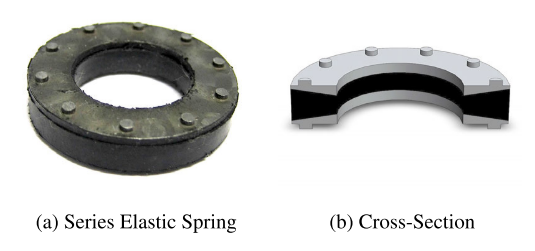
\includegraphics[width=0.6\textwidth]{RotarySoftSEA.png}
    \caption{Developed soft rotary spring: a)photo and b)cross-section \cite{rollinson2013design}.}
    \label{fig:rotarySoftSEA}
\end{figure}

Following a more traditional approach, Schepelmann et al. incorporated viscoelasticity in cable-driven SEA by using a rubber material as the elastic element, instead of the traditional metallic spring \cite{schepelmann2014compact}. In here, no LVMs are used, instead the non-linear stress response of the rubber is simplified by fitting a second order exponential curve to the stress-strain curve of the material. The main motivation of this work is to tackle the limitations of SEA with non-linear springs (NLS), where computer-aided manufactured (CAM) structures are used to define a known deflection trajectory of the spring, thus defining a torque trajectory. Essentially, CAM structures are able to relate the spring deformation with the generated torque, allowing the implementation of control systems. This work successfully validated the suitability of rubber to be incorporated as part of a SEA (\Cref{fig:softSEACAM}). However, under the limited range of testing parameters, the authors were not able to observe any velocity-dependency on the stress response of the rubber. In the conclusions, a state space observer is recommended to improve the accuracy of the reported forces transmitted by the the soft material, i.e. to allow the controller to compensate the hysteresis and non-linear stress response of the material.

\begin{figure}[htb!]
    \centering
    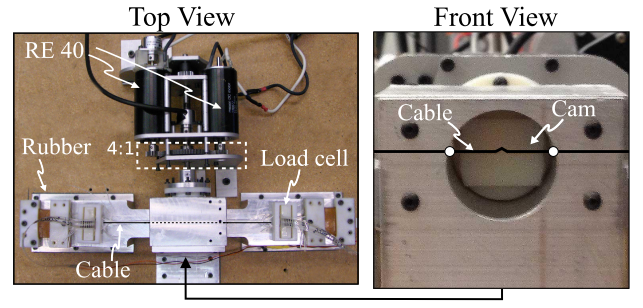
\includegraphics[width=0.6\textwidth]{SoftSEACAM.png}
    \caption{Benchtop setup for rubber characterization and observer testing. The load side of the rubber is fixed. Load cells in-line with the rubber give rubber force measurements for testing. The choice of electric motors and transmission is illustrated \cite{schepelmann2014compact}}
    \label{fig:softSEACAM}
\end{figure}

In an attempt to relieve the controller for such load, the latter work was continued by Austin et al. in \cite{austin2015control}, this time the focus was on developing a modelling tool to better model the complex behaviour of rubber. In here, the complexity of modelling the non-linear and strain-dependent stress response of soft materials is addressed, for the first time, by upgrading the SLS model without greatly increasing its complexity. A piecewise linearization method is implemented, to transform the equilibrium spring in the SLS model into several springs in parallel which sequentially engages in proportion to the strain applied to the material. The developed mathematical model is called the Standard Linear Solid model with Strain-Dependent Stiffness. (Std. Lin. SDS). Although, the SLS is not the most complete model among the LVM, the reported accuracy of the developed model is impressive. The control system implemented a state space observer, as well, which was able to correctly estimate the torque generated by the rubber spring. However, despite the large improvement in accuracy obtained by the developed Std. Lin. SDS, the hysteretic properties of the rubber  lead to instability at higher frequencies, suggesting that there is still work to be done in this field.

\section{Summary}

In this chapter, the terminology on the biomechanics of the human lower limb is presented. Subsequently, the characterization of the kinetic and kinematic parameters of the hip, knee and ankle joints is performed by reviewing many clinical trials about gait analysis of the lower limb. The collected data had the potential to be used as design guidelines when developing robotic devices targeted for human assistance. Therefore, many visualization techniques were proposed and analysed in this context. The latter work resulted in a published conference paper (\Cref{sec:characterizationKKP}). 

The main element of the human skeletal muscle system, the muscle-tendon component, was described in \Cref{sec:muscle_tendon}. In the literature, the works that implement the concept of mimicking the muscle skeletal system are focused on the contractile element of the muscle-tendon component, i.e. the muscle. Very little attention is paid to the series element, the tendon. Furthermore, it was found that the viscoelasticity present in the human tendon, and biological tissues in general, is also present in certain polymers and composite materials. Therefore, the proposal of performing a comparison analysis between different off-the-shelf composite materials and the human tendon mechanical properties is presented. This comparison analysis will contribute to the aforementioned aim of the research. The first step to perform this comparison analysis is to characterize the mechanical properties of the selected materials, listed in \Cref{sec:softMaterials}. This is described in \Cref{ch:characterizationSoft}.

Recently, attempts of adding viscoelasticity to well-established actuation technologies have been done. Specifically, viscoelasticity has the potential to address many of the limitations found in series-elastic actuators. The available literature on the subject is scarce but very well documented. In general, the reviewed works face a common challenge, the modelling of the viscoelastic properties of the materials used to accurately estimate their reaction force or torque. Rubber is the most common choice in these applications. Almost all of the documented works are based on a model-driven approach, based on the Linear Viscoelastic Models, for the prediction of the material behaviour. However, the work performed by Austin et al. in \cite{austin2015control}, is the first attempt to upgrade the potential of the LVMs by applying a piecewise linearization method. The authors succeeded in developing a mathematical model, called the Standard Linear Solid model with Strain-Dependent Stiffness. (Std. Lin. SDS) which achieved higher accuracy than traditional models. However, even with the aid of controlling techniques such as the state space observer, the implemented control system is still unable to account for properties of the material, such as hysteresis and the velocity-dependency in their stress response. Nevertheless, the developed mathematical model has the potential to be upgraded further by using the same piecewise linearization method but on a more complex LVM. This idea is further explored in an attempt to develop a reliable modelling tool for the prediction of the mechanical properties of soft materials. This is presented in \Cref{sec:ChapterModellingLVM}.


